
\documentclass[12pt,a4paper,twoside]{book}

% -------------------------------------------------
% PAQUETES
% -------------------------------------------------

\usepackage[utf8]{inputenc}
\usepackage[T1]{fontenc}
\usepackage[spanish]{babel}

\usepackage{graphicx}
\usepackage{float}
\usepackage{amsmath}
\usepackage{amssymb}
\usepackage{booktabs}
\usepackage{multirow}
\usepackage{array}
\usepackage{caption}
\usepackage{subcaption}
\usepackage{geometry}
\usepackage{setspace}
\usepackage{listings}
\usepackage{xcolor}
\usepackage[hidelinks]{hyperref}
\usepackage{comment}
\usepackage{url}
\usepackage[style=apa,backend=biber]{biblatex}
\usepackage{graphicx}
\usepackage{float}

\usepackage{xcolor}

\addto\captionsspanish{
  \renewcommand{\tablename}{Tabla}
  \renewcommand{\listtablename}{Índice de tablas}}

\newcommand{\todo}[1]{\textcolor{red}{[#1]}}

\raggedbottom
\addbibresource{bibliografia.bib}

% -------------------------------------------------
% CONFIGURACIÓN DE PÁGINA
% -------------------------------------------------
\usepackage{fancyhdr}

\pagestyle{fancy}

% Limpia cabecera y pie
\fancyhf{}

% Número de página en el exterior inferior (tipo libro)
\fancyfoot[LE,RO]{\thepage}

\renewcommand{\headrulewidth}{0pt}
\renewcommand{\footrulewidth}{0pt}

% Estilo para páginas de inicio de capítulo (IMPORTANTE)
\fancypagestyle{plain}{
    \fancyhf{}
    \fancyfoot[LE,RO]{\thepage}
    \renewcommand{\headrulewidth}{0pt}
}


\begin{comment}
\geometry{
    left=3cm,
    right=2.5cm,
    top=3cm,
    bottom=3cm
}
\end{comment}

% -------------------------------------------------
% INICIO DOCUMENTO
% -------------------------------------------------

\begin{document}

% -------------------------------------------------
% PORTADA
% -------------------------------------------------

\begin{titlepage}
		%Poner imagen del logo de comillas
		\centering
		\Large GRADO EN INGENIERÍA EN TECNOLOGÍAS DE TELECOMUNICACIÓN \\ % Modify accordingly
		\vspace*{2.5em} 
		\centering
		TRABAJO FIN DE GRADO\\ 
		\vspace*{1em}
		TITULO DEL TFG 
		\\ \large
		\vspace*{3em}
		Autor \\ Ana Arregui Beltrán \\ 
		\vspace*{1em}
		Director \\ Lucas Novales Peleato \\
		\vfill
		Madrid \\
		Junio 2026
\end{titlepage}

\cleardoublepage

\section*{Agradecimientos}

\newpage

% -------------------------------------------------
% RESUMEN Y ABSTRACT
% -------------------------------------------------
\section*{Título del TFG (español)}
\section*{Resumen}

\newpage

\section*{Título del TFG (inglés)}
\section*{Abstract}

\newpage

% -------------------------------------------------
% ÍNDICES
% -------------------------------------------------

\tableofcontents
\newpage

\listoffigures
\newpage

\listoftables
\newpage

% -------------------------------------------------
% CAPÍTULO 1
% -------------------------------------------------

\chapter{Introducción}

\section{Contexto del problema}


\section{Motivación}


\section{Problema a resolver}


\section{Objetivos}

\section{Alcance del proyecto}

Que hace, que no hace y limitaciones

\section{Estructura de la memoria}


% -------------------------------------------------
% CAPÍTULO 2
% -------------------------------------------------

\chapter{Fundamentos Teóricos y Tecnologías}

\section{Anatomía eléctrica del corazón}

El corazón es un órgano muscular que funciona como una bomba para impulsar la sangre a través del sistema circulatorio. Esta acción de bombeo está regulada por un sistema eléctrico, encargado de coordinar las contracciones de las distintas cavidades del corazón.

El latido se genera en la aurícula derecha, donde se encuentra el nodo sinoauricular (SA) que actúa como marcapasos natural del corazón. El nodo SA envía pulsos eléctricos que se propagan a través de las aurículas derecha e izquierda, llegando al nodo auriculoventricular (AV). En este nodo, el impulso disminuye brevemente, permitiendo que las aurículas se contraigan antes que los ventrículos. Así, la sangre se vacía de la aurículas a los ventrículos antes de su contracción.

Después de pasar por el nodo AV, la corriente eléctrica desciende por el Haz de His hasta los ventrículos. Esta vía se divide en dos ramas, derecha e izquierda, conocidas como ramas de His. Estas ramas estimulan electricamente los ventrículos derecho e izquierdo, provocando su contracción y el bombeo de la sangre hacia el exterior del corazón. (\cite{stanford_electrical_system})

\begin{figure}[H]
    \centering
    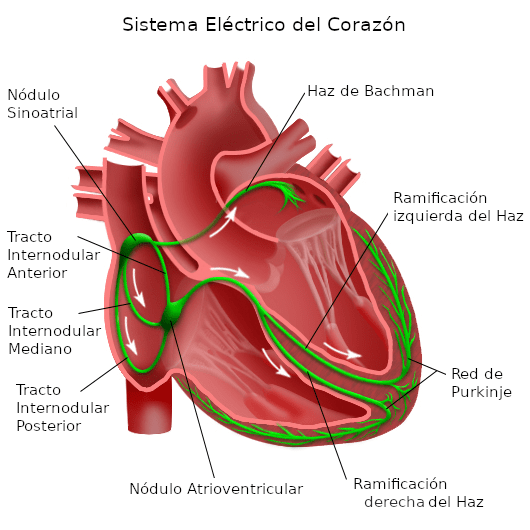
\includegraphics[width=0.4\textwidth]{imagenes/sistema-electrico-corazon.png}
    \caption{Anatomía eléctrica del corazón.}
    \label{fig:sistema-electrico-corazon}
\end{figure}

\footnote{\cite{cigna_corazon_electrico}}

\todo{Explicar la anatomía basica del corazon??}


\section{Electrocardiograma}

\subsection{¿Que es un ECG?}

El electrocardiograma (ECG) es la representación gráfica de la actividad eléctrica del corazón a lo largo del tiempo. Se trata de una prueba no invasiva, de bajo coste y fácil de realizar. Esta representación se utiliza para buscar actividad cardíaca anormal, que pueda indicar la presencia de patologías cardíacas. 

No solo se utiliza para diagnosticar enfermedades, sino que el ECG puede evaluar el ritmo cardíaco, si este es regular o irregular y la fuerza y sincronización de las señales eléctricas. Además, se puede medir el tamaño y la posición de las cavidades del corazón. (\cite{medlineplus_ecg_es}) 

El ECG es una herramienta fundamental en la práctica clínica, ya que permite la interpretación del ritmo cardíaco y la detección de alteraciones del sistema eléctrico. Aporta información relevante en la evaluación de patologías cardiovasculares, como valvulopatías, miocardiopatías, pericarditis, isquemia miocárdica o enfermedades hipertensivas. Por otro lado, el ECG se puede utilizar para monitorizar la respuesta a tratamientos farmacológicos, especialmente antiarritmicos, así como en la detección de alteraciones metabólicas. (\cite{prutkin_ecg_uptodate})

\subsection{Sistema de derivaciones del ECG}

Para medir la actividad eléctrica del corazón, se colocan electrodos en cada una de las extremidades y en el pecho, formando un sistema de 12 derivaciones. Cada derivación mide la diferencia de potencial eléctrico entre dos puntos o un punto del cuerpo y una referencia. El electrodo conectado en la pierna derecha sirve como electrodo de referencia a tierra. (\cite{cvphysiology_ecg_leads})

Existen dos tipos de derivaciones: las derivaciones bipolares y las derivaciones unipolares. Las derivaciones bipolares utiliza un electrodo positivo y otro negativo para medir la diferencia de potencial, mientras que las derivaciones unipolares utilizan un unico electrodo positivo y una combinación de otros electrodos como electrodo de referencia.

Las doce derivaciones se agrupan en tres categorías según su ubicación: las derivaciones de las extremidades (I, II, III), las derivaciones aumentadas de las extremidades (aVR, aVL, aVF) y las derivaciones precordiales (V1-V6).

\begin{itemize}
	\item \textbf{Derivaciones de las extremidades}
	
	Son las únicas derivaciones bipolares y se colocan en brazos y piernas. Miden la actividad eléctrica del corazón en el plano frontal. 
	
	\begin{itemize}
		\item \underline{Derivación I}: Tiene el electrodo positivo en el brazo izquierdo y el negativo en el brazo derecho, midiendo la diferencia de potencial entre ambos brazos.
		\item \underline{Derivación II}: Tiene el electrodo positivo en la pierna izquierda y el negativo en el brazo derecho, midiendo la diferencia de potencial entre ambos puntos.
		\item \underline{Derivación III}: Tiene el electrodo positivo en la pierna izquierda y el negativo en el brazo izquierdo, midiendo la diferencia de potencial entre ambos puntos.
	\end{itemize}
	Estas tres derivaciones forman un triángulo equilátero, conocido como el \textit{triángulo de Einthoven}, que representa la relación entre las derivaciones de las extremidades. Esta relación es tal que la suma de los impulsos eléctricos registrados en las derivaciones I y III es equivalente a la suma de los impulsos registrados en la derivación II:
	
	\begin{equation*}
		DII = DI + DIII
	\end{equation*}
	
	Esta ley se conoce como \textit{Ley de Einthoven} y constituye una base fundamental para la interpretación vectorial de la actividad eléctrica cardíaca y permite verificar la coherencia de las señales registradas. (\cite{myekg_derivaciones_cardiacas})

	\begin{figure}[H]
		\centering
		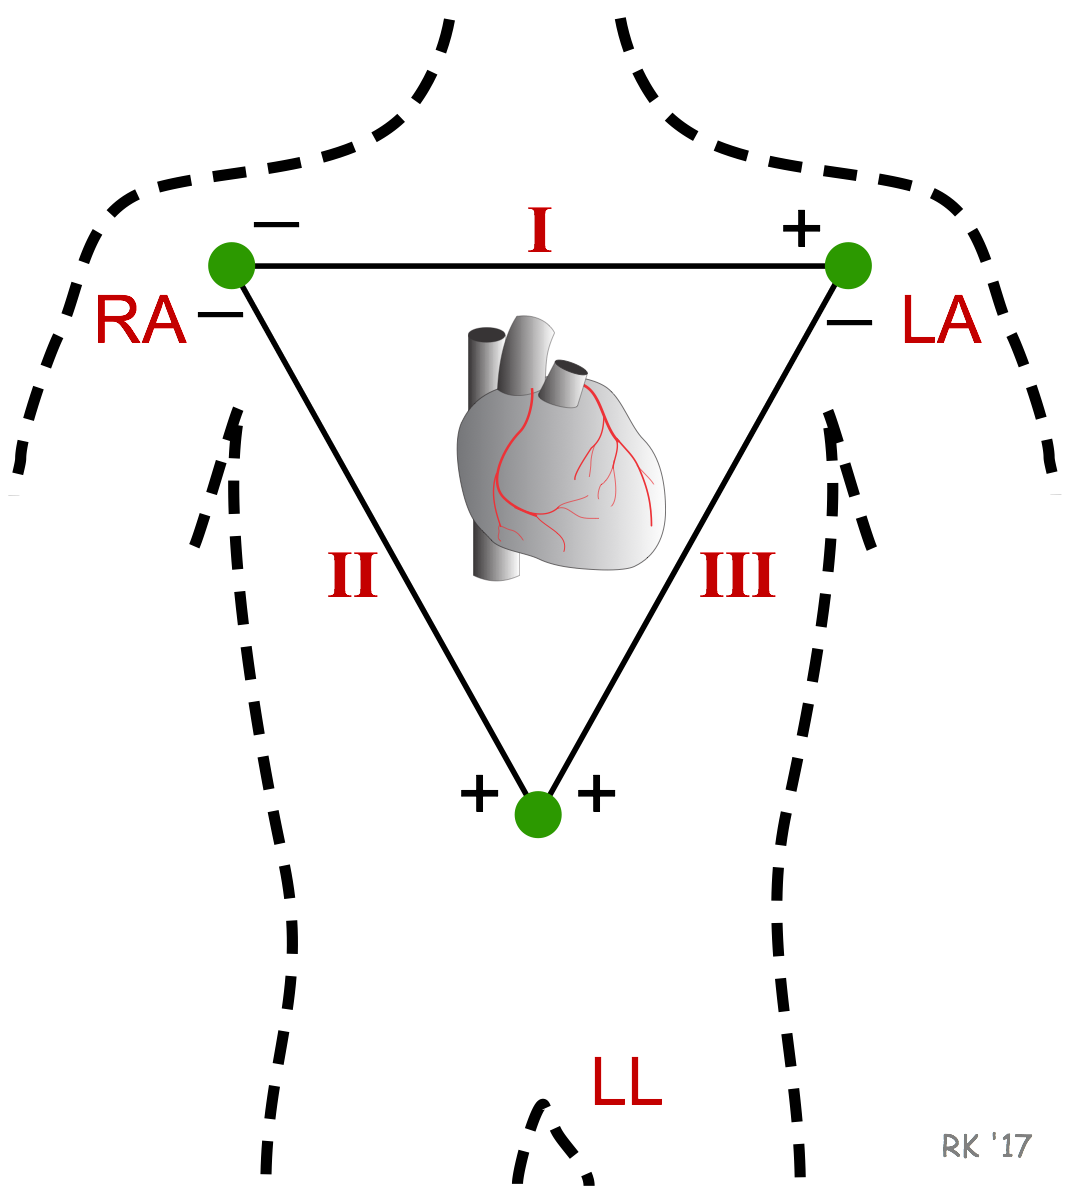
\includegraphics[width=0.3\textwidth]{imagenes/einthoven-triangle.png}
		\caption{Triángulo de Einthoven.}
		\label{fig:einthoven-triangle}
	\end{figure}

	
	\item \textbf{Derivaciones aumentadas de las extremidades}
	
	Se trata de derivaciones unipolares, que utilizan como referencia, una combinación de los electrodos de las extremidades. Al igual que estas, analizan la actividad eléctrica del corazón en el plano frontal.
	
	\begin{itemize}
		\item \underline{Derivación aVR}: El electrodo positivo está en el brazo derecho y mide la diferencia de potencial entre el brazo derecho y el centro del corazón.
		\item \underline{Derivación aVL}: El electrodo positivo está en el brazo izquierdo y mide la diferencia de potencial entre el brazo izquierdo y el centro del corazón.
		\item \underline{Derivación aVF}: El electrodo positivo está en la pierna izquierda y mide la diferencia de potencial entre la pierna izquierda y el centro del corazón.	
	\end{itemize}

	Estas derivaciones, complementan a las bipolares y permiten una visión más completa del plano frontal del corazón.

	\subsection*{Sistema hexaxial y eje del corazón}

	Si el triángulo de Einthoven se despliega y se superpone sobre el centro cardíaco, se puede definir un sistema de referencia angular que permite definir la dirección de la actividad eléctrica del plano frontal.

	Como se observa en la Figura \ref{fig:bipolar-limb-lead-axis} cada derivación bipolar tiene una orientación espacial:
	\begin{itemize}
		\item La derivación I se sitúa a 0º, correspondiente al eje horizontal entre el brazo derecho y el brazo izquierdo.
		\item La derivación II tiene una orientación aproximada de +60º con respecto a este eje horizontal, entre el brazo derecho y la pierna izquierda.
		\item La derivación III se orienta a +120º, entre el brazo izquierdo y la pierna izquierda.
	\end{itemize}

	Estas direcciones permiten interpretar la actividad eléctrica cardíaca como la proyección de un vector sobre distintos ejes espaciales. De este modo, el electrocardiograma no solo representa amplitudes eléctricas, sino también información direccional de la despolarización cardíaca. 

	\begin{figure}[H]
		\centering
		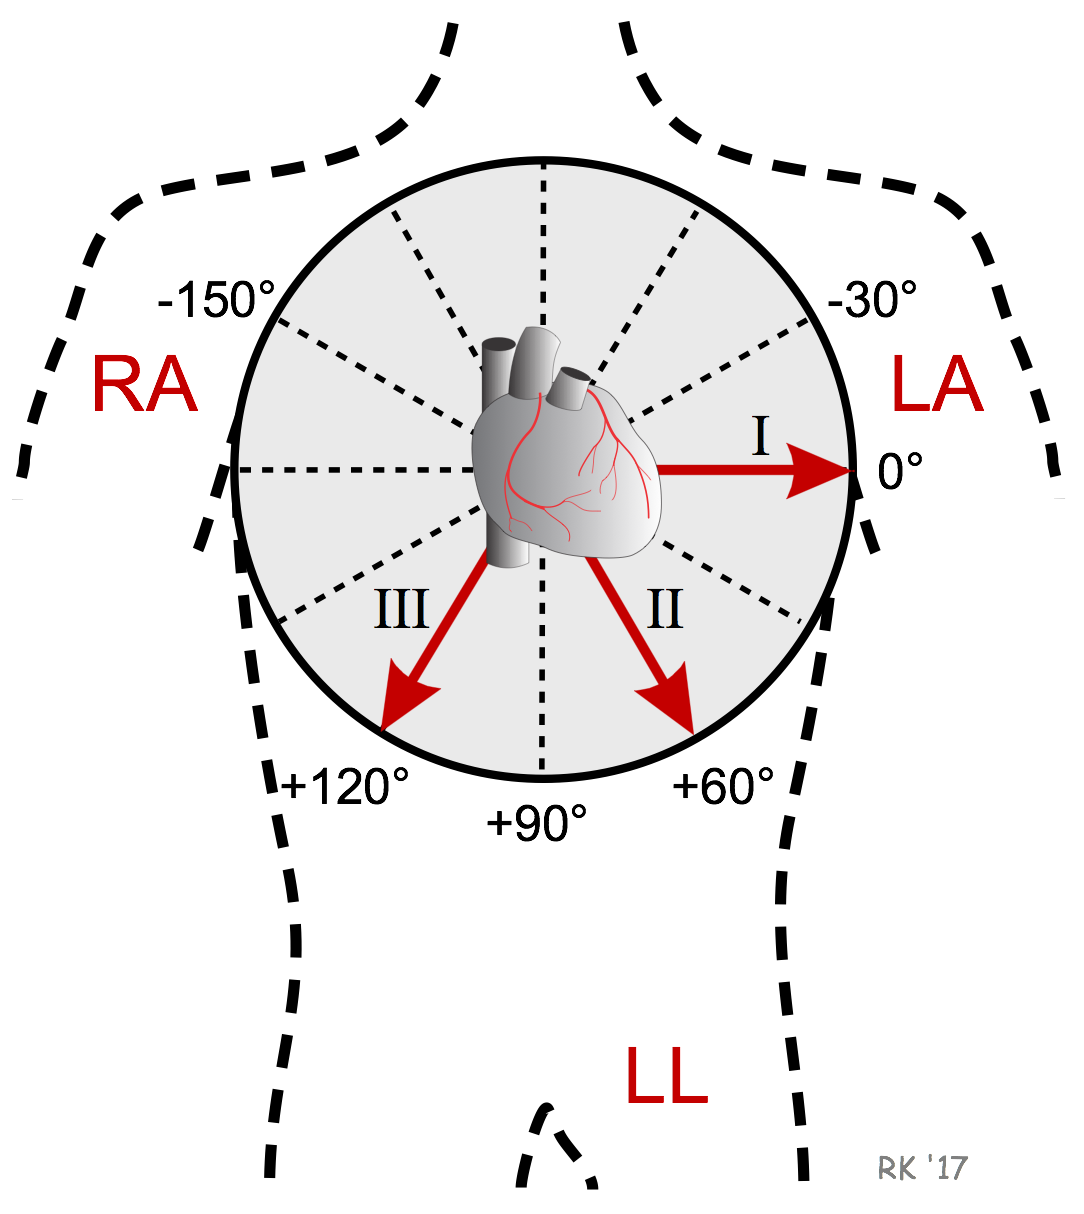
\includegraphics[width=0.3\textwidth]{imagenes/ecg-bipolar-limb-lead-axis.png}
		\caption{Eje de las derivaciones bipolares en el plano frontal}
		\label{fig:bipolar-limb-lead-axis}
	\end{figure}

	A partir de este sistema de derivaciones se incorporan las derivaciones aumentadas de las extremidades, que completan la cobertura del plano frontal y permiten una explicación más precisa del vector eléctrico. Estas derivaciones se sitúan en los siguiente ángulos:

	\begin{itemize}
		\item Derivación aVL: -30º sobre la horizontal
		\item Derivación aVR: -150º sobre el eje horizontal
		\item Derivación aVF: +90º sobre el plano horizontal
	\end{itemize}

	\begin{figure}[H]
		\centering
		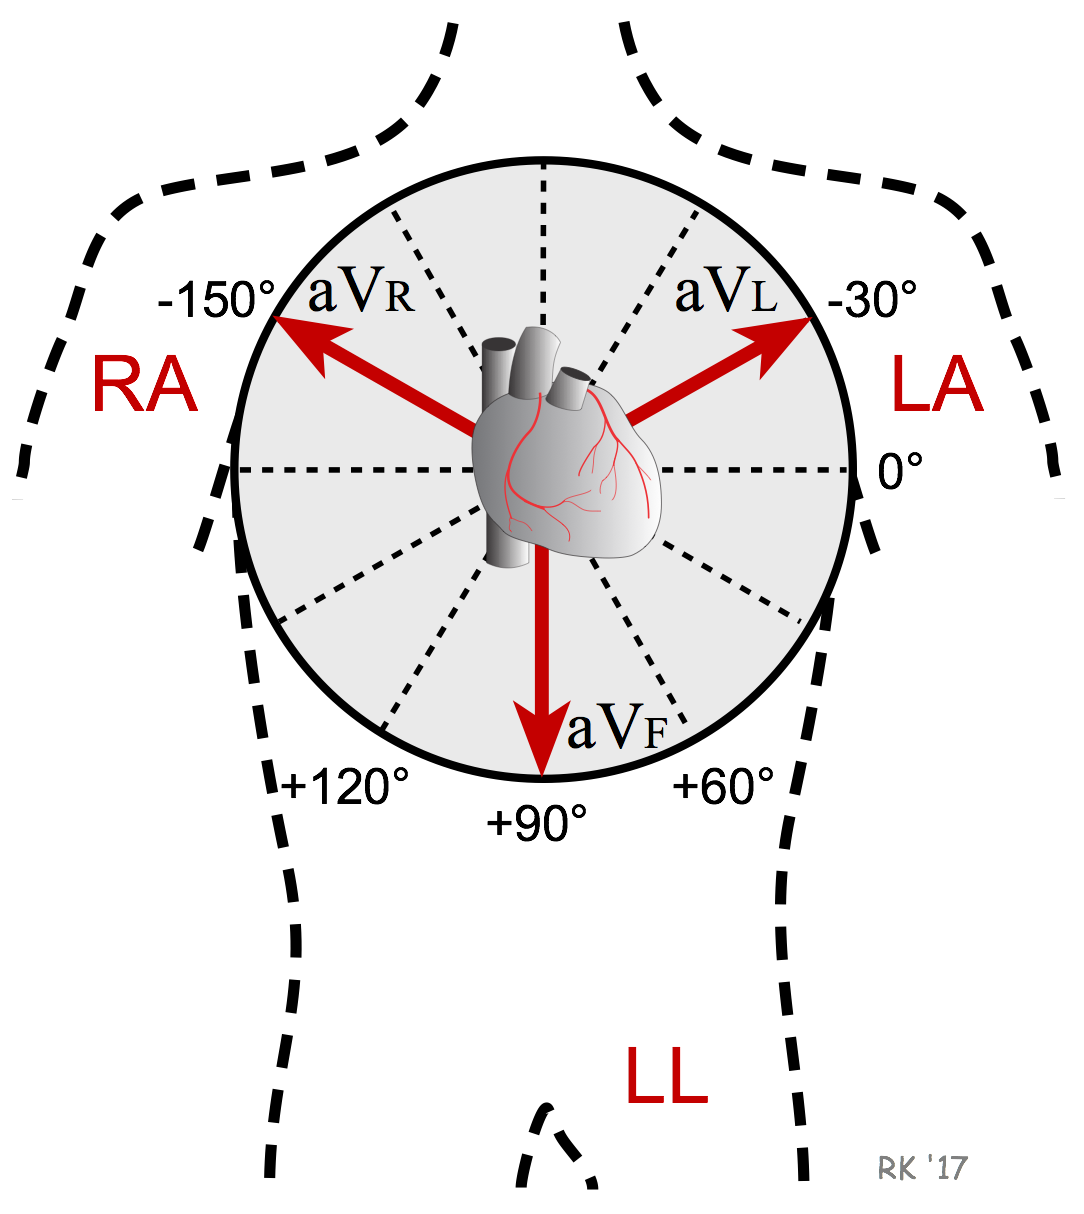
\includegraphics[width=0.3\textwidth]{imagenes/ecg-augmented-lead-axis.png}
		\caption{Eje de las derivaciones aumentadas de las extremidades en el plano frontal}
		\label{fig:augmented-limb-lead-axis}
	\end{figure}

	El conjunto de estas seis derivaciones constituye el sistema hexaxial completo, que permite analizar la dirección del vector eléctrico cardíaco en el plano frontal y constituye la base para la determinación del eje eléctrico del corazón.

	\begin{figure}[H]
		\centering
		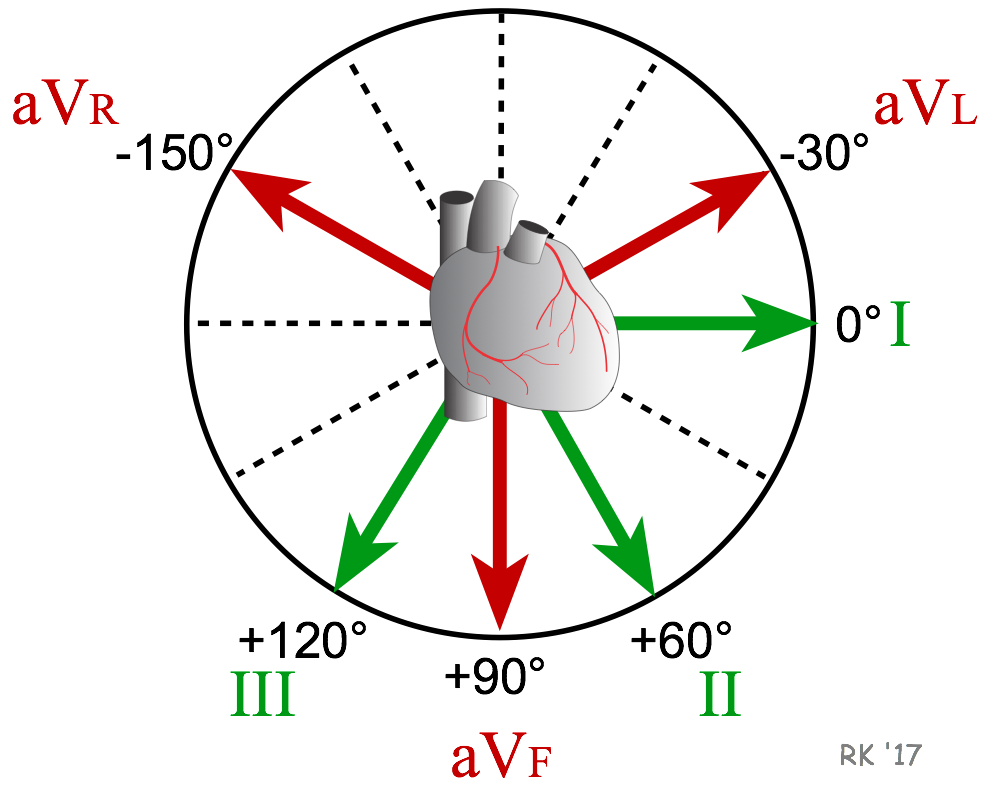
\includegraphics[width=0.3\textwidth]{imagenes/ecg-6-limb-lead-axis.png}
		\caption{Sistema hexaxial}
		\label{fig:sistema-hexaxial}
	\end{figure}
	
	Este eje se determina a partir del complejo QRS (ver apartado \ref{sec:partes_ecg}), que representa la suma vectorial de todos los vectores eléctricos generados por la despolarización ventricular. Analizando la polaridad del QRS en las derivaciones del plano frontal, es posible determinar la dirección estimada de la actividad eléctrica cardíaca.
	En la práctica clínica, las derivaciones I y aVF son las más utilizadas para hacer una estimación rápida del eje eléctrico. 

	La determinación del eje se basa en la polaridad del complejo QRS en estas derivaciones. Cuando el vector de despolarización se dirige hacia el polo positivo de una derivación, la deflexión del complejo QRS es positiva; por el contrario, si el vector se aleja, la deflexión es negativa. (\cite{cardioteca_eje_cardiaco})

	El eje cardíaco en condiciones normales se encuentra entre -30º y 90º, haciendo que el vector resultante apunte abajo y a la izquierda. En este caso, el complejo QRS es positivo tanto en DI como en aVF. 

	
	
	En la tabla \ref{tab:eje_cardiaco} se resume la interpretación del eje cardíaco en función de la polaridad del complejo QRS en las derivaciones I y aVF.


	\begin{table}[H]
	\centering
	\caption{Interpretación del eje cardíaco según las derivaciones DI y aVF (\cite{prutkin_ecg_uptodate})}
	\label{tab:eje_cardiaco}

	\begin{tabular}{|c|c|c|c|c|}
	\hline
	\textbf{DI} & \textbf{aVF} & \textbf{Cuadrante} & \textbf{Rango del eje} & \textbf{Interpretación} \\ \hline

	+ & + & Inferior izquierdo & $-30^\circ$ a $+90^\circ$ & Eje normal \\ \hline

	+ & - & Superior izquierdo & $-30^\circ$ a $-90^\circ$ & Desviación izquierda del eje \\ \hline

	- & + & Inferior derecho & $+90^\circ$ a $+180^\circ$ & Desviación derecha del eje \\ \hline

	- & + & Superior derecho & $-90^\circ$ a $-180^\circ$ & Eje extremo derecho o izquierdo \\ \hline

	\end{tabular}
	\end{table}

	\item \textbf{Derivaciones precordiales}
	
	Estas seis derivaciones unipolares se colocan en el pecho, en diferentes regiones del corazón, y miden la actividad eléctrica en un plano perpendicular al plano frontal. Cada una de las derivaciones precordiales observa una región específica del ventrículo.
	
	\begin{itemize}
		\item \underline{Derivaciones V1-V2}: Exploran la region septal y anteroseptal del corazón, observando principalmente el septo interventricular.
		\item \underline{Derivaciones V3-V4}: Exploran la región anterior del corazón y el apex cardíaco, observando principalmente la pared anterior del ventrículo izquierdo.
		\item \underline{Derivaciones V5-V6}: Exploran en la región lateral y anterolateral izquierda del corazón, observando principalmente la pared lateral del ventrículo izquierdo.
	\end{itemize}

	\begin{figure}[H]
		\centering
		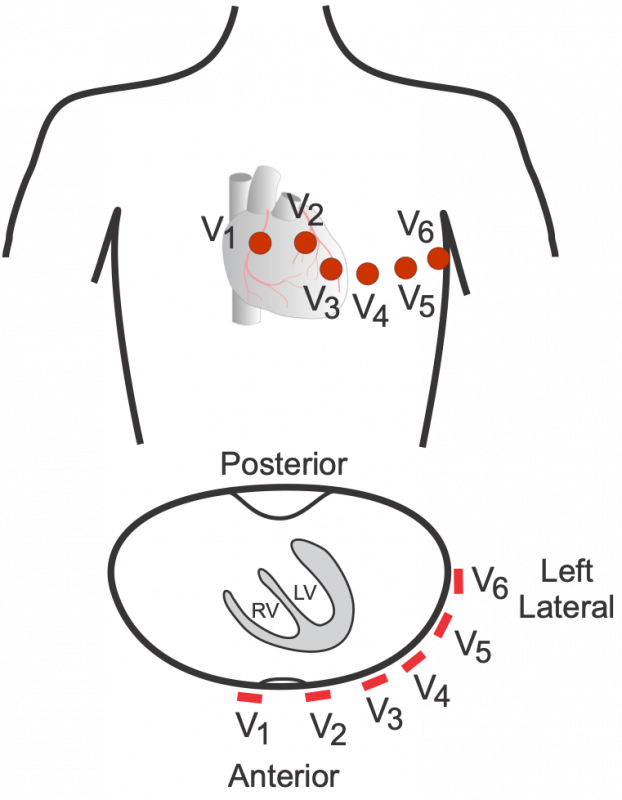
\includegraphics[width=0.3\textwidth]{imagenes/ecg-chest-leads.png}
		\caption{Derivaciones precordiales.\todo{poner pie de pagina con la fuente}}
		\label{fig:chest_leads}
	\end{figure}

\end{itemize}

\subsection{Partes del ECG}
\label{sec:partes_ecg}

Un ciclo cardíaco típico en el ECG está compuesto por varias ondas y segmentos característicos, cada uno de los cuales se asocia a una fase concreta del proceso eléctrico del corazón.

\subsubsection{Onda P}

La onda P representa la despolarización de las auriculas. En la mayoría de las derivaciones es positiva, salvo en aVR

\subsection{}

derivaciones, ondas, alteraciones



\section{Patologías estudiadas}

Explicar las 5 patologias grandes

\section{Machine Learning}



\section{Clasificación multilabel}



\section{Métricas de evaluación}

Todas las metricas Accuracy, precision recall etc

\section{Tecnologías y librerías utilizadas}

% -------------------------------------------------
% CAPÍTULO 3
% -------------------------------------------------

\chapter{Estado del Arte}

Ampliar considerablemente el estado del arte del anexo B

IA aplicada al diagnostico cardiaco

Trabajos relacionados

Limitaciones de los trabajos relacionados

Justificacion del proyecto-> O lo pongo en el capitulo 4?


% -------------------------------------------------
% CAPÍTULO 4
% -------------------------------------------------

\chapter{Definición del Trabajo}

\section{Justificación del proyecto}

Aqui o en el 3?

\section{Base de datos utilizada}

\subsection{Origen del dataset}


\subsection{Estructura del dataset}


\subsection{Etiquetado original}


\subsection{Problemas del dataset}



\section{Agrupación de patologías}


\section{Escenarios experimentales}

\subsection{Enfoque 1}

1 derivacion + 5 clases + binario

\subsection{Enfoque 2}

12 derivaciones + 5 clases + binario

\subsection{Enfoque 3}

12 derivaciones + 71 clases + probabilidad

\section{Objetivos técnicos}

Thresholds, datos normales vs caracterisiticas, derivaciones

\section{Metodología general}



% -------------------------------------------------
% CAPÍTULO 5
% -------------------------------------------------

\chapter{Modelo Desarrollado}

\section{Arquitectura general del sistema}

Entradas, salidas, procesado de datos

\section{Análisis exploratorio de datos}

Distribución de clases, balanceo, correlaciones, etc

\section{Preprocesado de datos}

Limpieza, picos R, transformadas 

\section{Selección y extracción de características}

Justificar porque se han seleccionado esas características

\section{Desarrollo experimental y optimización del sistema}

Hablar aqui de todo: los modelos que he usado, los tres enfoques distintos 


% -------------------------------------------------
% CAPÍTULO 6
% -------------------------------------------------

\chapter{Análisis de Resultados}

Resultados globales, comparacion entre enfoques, resultados por enfermedad (matrices de confusion), thresholds personalizados, analisis clinicos, limitaciones

% -------------------------------------------------
% CAPÍTULO 7
% -------------------------------------------------

\chapter{Conclusiones y Trabajos Futuros}

Conclusiones y posibles mejoras y trabajos futuros

% -------------------------------------------------
% BIBLIOGRAFÍA
% -------------------------------------------------

\cleardoublepage
\addcontentsline{toc}{chapter}{Bibliografía}

\nocite{*}
\printbibliography
% -------------------------------------------------
% ANEXOS
% -------------------------------------------------
% Añadir anexos pertinentes
\end{document}